\subsection{Which PMU Can Distinguish a Short Torque Pulse?}
\label{app:torque-terminal}

A positive torque pulse can end before its source is clear. The rotor
angle continues to evolve after the torque returns to nominal. We use
that motion to locate a first pulse from steady operation. Azizi
\emph{et al.} locate generation losses from the voltage and current
changes associated with a change of nodal injection
\cite{azizi2021log}. Here the generator stays connected. A finite
mechanical input drives the swing equations through its own rotor,
and the question is how soon the observed trajectory distinguishes
its bus from another generator.

Let $A_h$ and $B_h$ be the discretized swing and governor dynamics
and the torque-input map for inertia multiplier $h$. The source
vector $e_g$ selects generator $g$. For onset $\tau$, duration $d$
and unit severity, the physical response satisfies
\[
 x_{t+1}=A_h x_t+B_h e_g\,\mathbf{1}_{\{\tau\le t<\tau+d\}},
 \qquad s_{t}=H x_{t+1},\qquad x_\tau=0 .
\]
The columns of $B_h$ include the nominal torque increment. The
voltage rows of $H$ map rotor angles through the network equations
to log magnitudes and voltage angles at the eight PMUs. At an
energized terminal with nominal outward current $I_0$, the additional
current-angle row follows from
$\delta\arg I=\operatorname{Im}(\delta I/I_0)$ with
$\delta I=Y_{\rm term}\delta V$. Both models standardize the voltage
coordinates by their quiet training scales. For the terminal angle
we assign a standard deviation of $10^{-3}$ rad.

\paragraph{A comparison on the same reports.}
Stack the first $N$ reports in $y$ and place the predicted response
$s$ on those same reports, padding with zeros before its onset.
Assume independent standardized Gaussian errors and an unknown
constant reference for each channel. Let $P_N$ subtract the temporal
mean of each channel. Integrating the reference with a common flat
prior gives the log likelihood ratio for severity $a$ against a
quiet trajectory,
\begin{equation}
 L_N(a,s)=a\langle P_Ns,P_Ny\rangle
              -\tfrac12 a^2\|P_Ns\|^2 .
 \label{eq:pulse-common-prefix}
\end{equation}
This follows by completing the square in the reference in both
Gaussian likelihoods. Their normalizing factors cancel. At a report
where the fast scan crosses threshold, every generator competes on
the same $y$, including the part of the record that a later-onset
candidate predicts was quiet. Its evidence is the prior-weighted
sum of $\exp L_N$ over onset, inertia, duration and severity. With
equal generator priors and equal costs for incorrect buses, the
largest of these sums minimizes conditional source error under the
specified finite model.

The reader searches ages 1--45 reports on a three-report decision
clock, with equal discrete prior masses on inertia multipliers
$\{0.8,1,1.2\}$, durations $\{7,9,18,45\}$ and positive severities
$\{0.75,1,1.25\}$. Its four screening windows span 9, 15, 24 and
36 reports, each following a 45-report local reference. With
$K=30\times86400/0.01$, the screen requires a generator-mixture
likelihood ratio above $4K$, and the common-prefix
mixture must exceed $K$. The largest conditional generator
probability must exceed 0.99. The residual over the last 45 reports
at the best-fitting setting for that bus must also fall below the
0.99999 quantile of a chi-squared reference with $45p$ degrees of
freedom for $p$ coordinates. These checks define the implementation's
alarm policy. The conditional optimality of the bus decision does
not establish an optimal stopping rule or an operational false-alarm
rate.

The four-family bank continues processing the stream. Its first
publication disarms the torque reader and has priority at a tied
time. If the reader has already published, a bank torque alarm whose
estimated onset lies within 12 reports of the first estimate and
whose publication lies within its 45-report deadline is merged with
that declaration. Other bank alarms pass through. This logic leaves
second-event decisions after a first fault or line opening with the
original bank.

\paragraph{Selecting the current terminal.}
For a nominal seven-report pulse at bus $i$, compare its predicted
trajectory with that of a rival $j$. Give the rival its most favorable
onset, duration, inertia and severity. For a given rival template
$s_j$, the least-squares severity is
\[
 a^*=\operatorname{clip}_{[0.75,1.25]}
 \frac{\langle P_Ns_i,P_Ns_j\rangle}{\|P_Ns_j\|^2}.
\]
When the denominator vanishes, severity drops out. Let $D_i$ be the
smallest $\|P_N(s_i-a^*s_j)\|$ over rival templates at other buses.
For the resulting pair of fixed Gaussian means with equal prior
probabilities, the optimal binary decision errs with probability
$\Phi(-D_i/2)$. The scalar decision statistic along the difference
of the whitened means has unit variance and means $\pm D_i/2$.
Therefore, a pair with $D_i<3.29$ precludes 95\% correct decisions
for both members uniformly over the allowed reference offsets and
pulse settings. This is a two-hypothesis design calculation for the
specified noise law. It does not estimate a ten-generator error rate.

\begin{figure}[t]
\centering
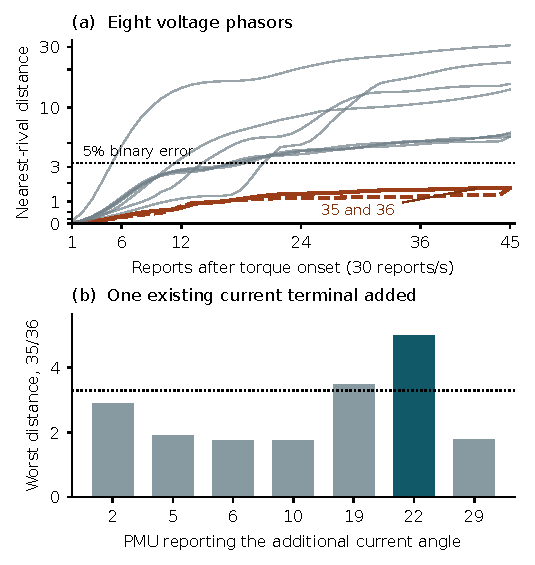
\includegraphics[width=\columnwidth]{figures/generated/torque_terminal_design.pdf}
\caption{Source separation for a nominal seven-report pulse, allowing
a rival generator to change its onset, duration, inertia and severity.
The upper panel shows the ten voltage-only distances, with a
compressed scale at large distances. The lower panel shows the
smaller distance for buses 35 and 36 at 45 reports when one existing
current angle is added with independent $10^{-3}$-rad noise. The
dotted line marks 5\% error in the two-mean Gaussian decision.}
\label{fig:torque-terminal-design}
\end{figure}

With voltage alone, the closest pair at the deadline is buses 35 and
36 (Fig.~\ref{fig:torque-terminal-design}). We evaluated each of the
seven available current angles in the same distance calculation and
selected the terminal maximizing the smaller distance for those two
buses. The selected current is measured at bus 22 on branch 21--22.
The choice uses the network model, candidate catalog and assumed noise
scales. It requires no source-labeled PMU record from either bus.

\begin{table}[t]\centering\footnotesize
\caption{Frozen four-family replication on 465 new streams and 420 events. Exact requires both family and asset within 45 reports. Active counts exact decisions published before clearance. Extra counts unmatched alarms throughout the records.}
\label{tab:torque-terminal-trial}
\setlength{\tabcolsep}{2.5pt}
\begin{tabular*}{\columnwidth}{@{\extracolsep{\fill}}lrrrrr@{}}\toprule
Monitor & Macro-F1 & Family & Exact & Active & Extra\\\midrule
Recovery bank & 0.968 & 400 & 396 & 386 & 7 \\
With voltage reader & 0.972 & 405 & 401 & 391 & 8 \\
With terminal reader & 0.977 & 410 & 406 & 391 & 9 \\
Refitted ExtraTrees & 0.699 & 267 & 258 & 94 & 7 \\
\bottomrule\end{tabular*}\end{table}


Both readers passed the development criterion of increasing joint
diagnoses and macro-F1 without increasing unmatched alarms over the
bank on either of two development cohorts. Both exceeded the trees'
unmatched-alarm counts in development. We froze the voltage reader
for the primary incremental comparison and froze the terminal reader
as a separate comparison before generating the new test records. The
15 new scenario blocks draw times, strengths, parameters and noise
on the same reserved asset catalog. The eight PMUs, publication
deadline and matching rule are common to all methods. Paired
95\% percentile intervals resample the 15 whole blocks, including the
nominal and variable-governor trajectories together.

Table~\ref{tab:torque-terminal-trial} gives the continuous results.
Against the original bank, the paired intervals for the change in
joint accuracy (percentage points) were
$[\TorqueVoltBaseGainCI]$ for the voltage reader and
$[\TorqueTermBaseGainCI]$ for the terminal reader. The interval for
adding the terminal to the voltage reader was $[\TorqueTermVoltGainCI]$.
The terminal recovered six short pulses at bus 35, lost one timely
diagnosis at bus 32 and matched the voltage reader at bus 38. Each
bus contributed ten pulses from five paired scenario blocks.
Of 30 isolated short pulses, the bank, voltage reader and terminal
reader located \TorqueBaseShort{}, \TorqueVoltShort{} and
\TorqueTermShort{} within the deadline. They located
\TorqueBaseShortActive{}, \TorqueVoltShortActive{} and
\TorqueTermShortActive{} before the pulse ended. These endpoints
distinguish recognizing the motion left by a pulse from identifying
the source while torque is still applied.

To check the assumed noise scale, we replayed the terminal reader
alone on the 24 isolated short pulses from the two development
cohorts. We added independent Gaussian angle errors at terminal 22,
using the same standardized noise realization at each level. At
added standard deviations of 0, 1, 2 and 5~mrad, the reader located
\TorqueStressZero{}, \TorqueStressOne{}, \TorqueStressTwo{} and
\TorqueStressFive{} pulses within the deadline. It remained silent on
all 36 quiet controls at every level. Voltage reports were identical
across these runs. This sensitivity check evaluates the first-event
reader alone on development records.
